\documentclass{beamer}

\mode<presentation> {	
	%\usetheme{Antibes} %ok
	%\usetheme{Berlin} %ok
	%\usetheme{Boadilla} %ok
	\usetheme{Darmstadt} %ok
	%\usetheme{Dresden} %ok
	%\usetheme{Frankfurt} %ok
	%\usetheme{Ilmenau} %ok
	%\usetheme{Pittsburgh} %ok
	%\usetheme{Rochester} %ok
	
	
	%\usecolortheme{dolphin}
	%\usecolortheme{orchid}
	%\usecolortheme{whale}
}
\usepackage[utf8]{inputenc}
\usepackage[OT4]{polski}
\usepackage{tabularx}
\usepackage{graphicx} % Allows including images
\usepackage{booktabs} % Allows the use of \toprule, \midrule and \bottomrule in tables
\usepackage{verbatim}


\title[Modelowanie klimatu]{Modelowanie klimatu} % The short title appears at the bottom of every slide, the full title is only on the title page

\author{Axel Zuziak, Marcin Węglarz} % Your name
\institute[Akademia Górniczo-Hutnicza, WFiIS]
{
AGH WFiIS \\
Fizyka Techniczna\\ % Your institution for the title page
\medskip
}
\date{\today} % Date, can be changed to a custom date

\begin{document}
%progress bar in footline *************************************************************************

\definecolor{lightgr}{rgb}{0 0.4 0.9}
\makeatletter
\addtobeamertemplate{footline}{%
	\color{lightgr}% to color the progressbar
	\hspace*{-\beamer@leftmargin}%
	%\rule{\beamer@leftmargin}{0pt}%
	\rlap{\rule{\dimexpr
			\beamer@startpageofframe\dimexpr
			\beamer@rightmargin+\textwidth\relax/\beamer@endpageofdocument}{3pt}} %grubosc paska
	% next 'empty' line is mandatory!
	
	\vspace{0\baselineskip}
	{}
} %koniec progress bara **************************************************************************************



%++++++++++++++++++++++++++++++++++++++++++++++++++++++++++++++++++++++++
%notatki
%str 47-63
%str 117-150
%str 165-200
%str 244-246

%++++++++++++++++++++
%s.176
%TODO
%Fizyka + równania
%Implementacja tych równań 
%Typy modeli (0,1,2,3 wymiarowe + kompletne)
%s.60








\begin{frame}
\titlepage % Print the title page as the first slide
\end{frame}

%\begin{columns}[c]
%\column do  robienia kolumn
%\end{columns}

%\begin{frame}
%\frametitle{Overview} % Table of contents slide, comment this block out to remove it
%\tableofcontents % Throughout your presentation, if you choose to use \section{} and \subsection{} commands, these will automatically be printed on this slide as an overview of your presentation
%\end{frame}

%----------------------------------------------------------------------------------------
%	PRESENTATION SLIDES
%----------------------------------------------------------------------------------------

%------------------------------------------------
%\section{First Section} % Sections can be created in order to organize your presentation into discrete blocks, all sections and subsections are automatically printed in the table of contents as an overview of the talk
%------------------------------------------------

%\subsection{Subsection Example} % A subsection can be created just before a set of slides with a common theme to further break down your presentation into chunks
%--------------------------%
% Axel - slajdy -----------%
%--------------------------%
%----- Co to jest klimat? -%
%----- Ważne pojęcia ------%
%----- Model zerowymiarowy %
%----- Modelowane zjawiska fizyczne( atmostfera, ocean) -%
%----- Sprzężenia zwrotne i parametryzacja --------------%
%----- Rodzaje modeli + streszczenie --------------------%
%----- Implementacja GCM --------------------------------%

\begin{frame}
\frametitle{Co to jest klimat?}
\theoremstyle{definition}
\begin{block}{Klimat}
	Klimatem nazywamy średnie warunki pogodowe obserwowane w danym miejscu na przestrzeni lat. 
\end{block}
Modele klimatu są uproszonym opisem skomplikowanych procesów.

\begin{columns}
\begin{column}{0.5\textwidth}

	\textbf{Klimat dzielimy na:}
	\begin{itemize}
		\item Atmosfera %Gazowa część ponad powierzchnią ziemi.
		\item Hydrosfera %Wszystkie formy wody nad i pod powierzchnią ziemi.
		\item Kriosfera %Wszystkie formy wody w postaci lodu.
		\item Powierzchnia lądowa
		\item Biosfera %Organizmy żyjące w hydrosferze oraz na powierzchni lądowej.
	\end{itemize}
\end{column}
\begin{column}{0.5\textwidth}

	\textbf{Składniki klimatotwórcze:}
	\begin{itemize}
		\item Temperatura
		\item Opady
		\item Zachmurzenie
		\item Wilgotność
		\item Wiatr
	\end{itemize}
\end{column}
\end{columns}
\end{frame}


\begin{frame}
	\frametitle{}
	\begin{figure}[h]
		\begin{center}
			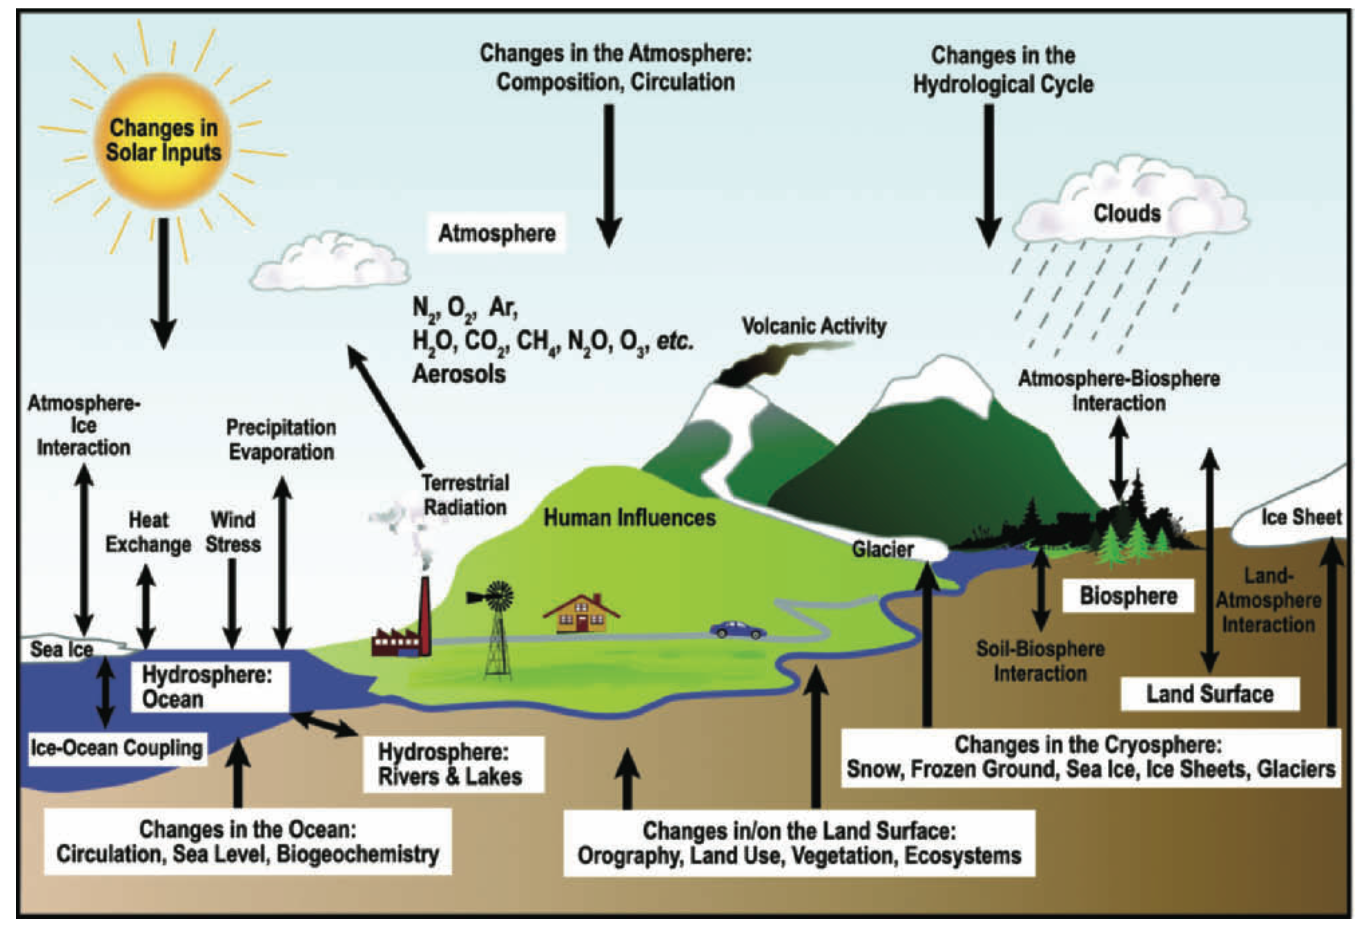
\includegraphics[width=0.9\linewidth]{images/Figure1}
			\caption{Czynniki definiujące i wpływające na klimat. [1]}
		\end{center}
	\end{figure}
\end{frame}

\begin{frame}
	\frametitle{Tworzenie modelu klimatu}
	\begin{figure}[h]
		\begin{center}
			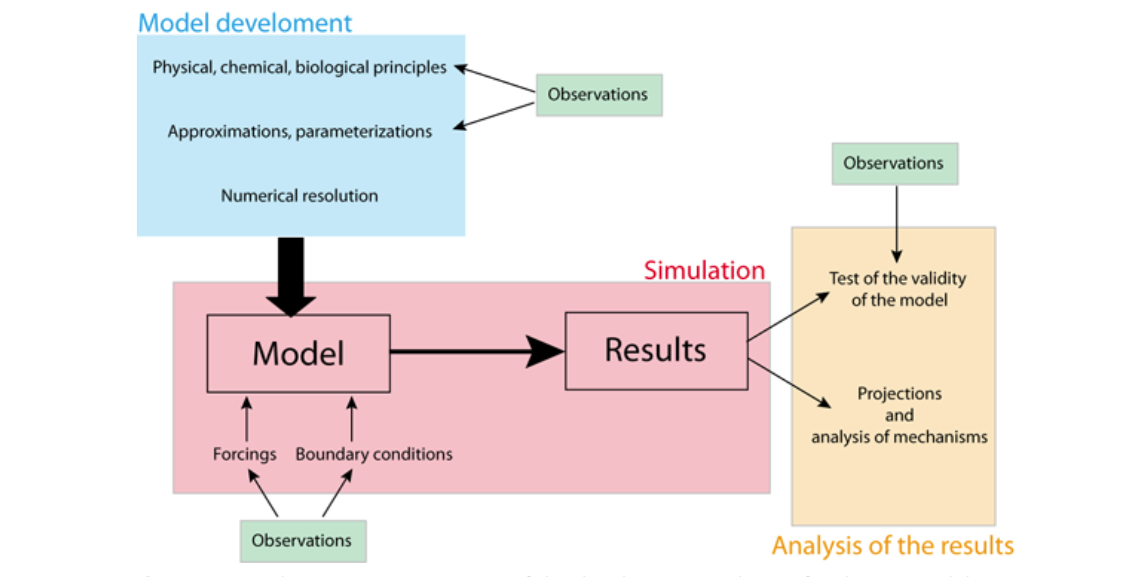
\includegraphics[width=1.0\linewidth]{images/Figure9}
			\caption{Proces tworzenia i weryfikowania modelu klimatu. [7]}
		\end{center}
	\end{figure}
\end{frame}

\begin{frame}
	\frametitle{Podział modeli}
	Ogólnie modele klimatu możemy podzielić na:
	\begin{itemize}
		\item zerowymiarowe
		\item 1-wymiarowe
		\item 2-wymiarowe
		\item 3-wymiarowe
	\end{itemize}
	\vspace{0.5cm}
	Spośród powyższych najdokładniejsze są modele 3-wymiarowe, z których należy wyróżnić
	\begin{itemize}
		\item GCM (general circulation model), AGCM,OGCM,CGCM lub AOGCM
		\item RCM (regional climate model)
	\end{itemize}
	
\end{frame}



\begin{frame}
	\frametitle{Zerowymiarowy model cieplarniany}
	\begin{figure}[h]
		\begin{center}
			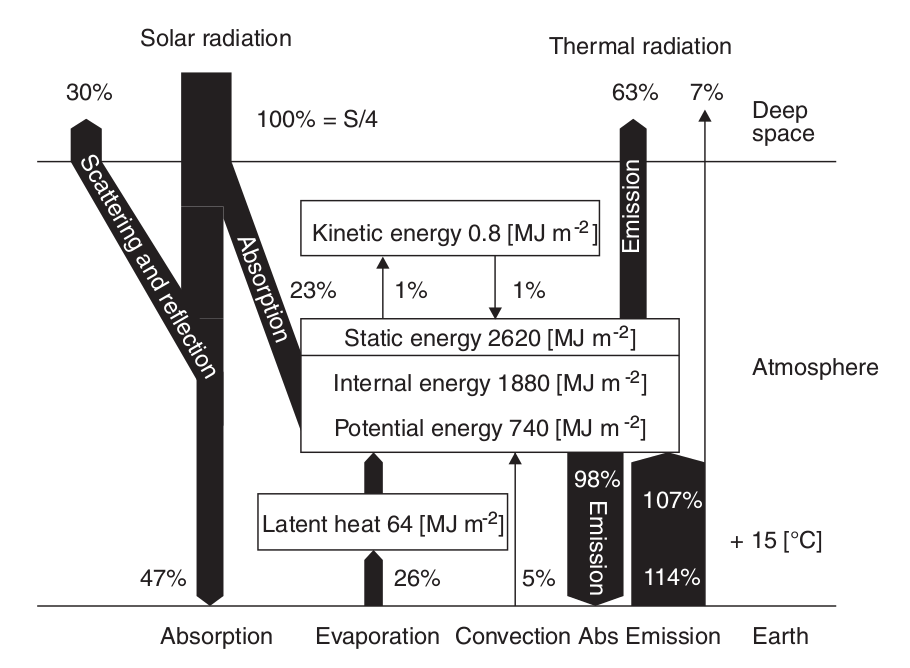
\includegraphics[width=0.7\linewidth]{images/0D_Model.png}
			\caption{Zerowymiarowy model bilansu promieniowania.\cite{b2}}
		\end{center}
	\end{figure}

\end{frame}



\begin{frame}
	\frametitle{Matematyczne spojrzenie na bilans energetyczny}
	\begin{block}{Bardzo prosty model bilansu radiacyjnego}
		\[(1-a)\frac{S}{4} = \sigma T_a^4 + t\sigma T_s^4
		\]
	\end{block}
	\begin{block}{Bilans dla powierzchni Ziemi}
		\[(-t_a)(1-a_s)\frac{S}{4}+c(T_s - T_a)+\sigma T_s^4(1-a_a^{'})
		-\sigma T_a^4 =0
		\]
	\end{block}
	\begin{block}{Bilans dla atmosfery}
		\[-(1- a_a-t_a+a_st_a)\frac{S}{4} - c(T_s - T_a) - \sigma T_s^4
		(1-t_a^{'}-a_a^{'}) + 2\sigma T_a^4=0
		\]
	\end{block}
	%Literką \it{a} oznaczamy albedo, natomiast \it{t} oznacza przepuszczalność. 
	%odpowiednie indeksy oznaczają wartość dla atmosfery(a) lub powierzchni Ziemi(s).
	\scriptsize{(Wartości z primem to wartości dla fal długich.)}
	
\end{frame}


\begin{frame}
	\frametitle{Wymuszenie radiacyjne i sprzężenie zwrotne}
	\textbf{Wymuszeniem radiacyjnym} nazywamy zjawisko zmiany temperatury na powierzchni Ziemi celem wyrównania bilansu radiacyjnego. 
	\begin{block}{Wzory do ilościowego opisu zmian temperatury}
		\[\Delta I = \frac{\partial I}{\partial T_s}\Delta T_s
		\]
		\[\frac{\partial I}{\partial T_s} = \frac{4}{T_s}(1-a)\frac{S}{4}
		\]
		
		%z tego modelu dI 3,1 W/m(-2)K(-1)
		%z dokladniejszych 4,6 - efekt uwzglednienia sprzezenia zwrotnego
	\end{block}
\end{frame}

\begin{frame}
	\frametitle{Modelowanie atmosfery}
	\begin{columns}
\begin{column}{0.5\textwidth}
		\begin{block}{Prawo zachowania pędu}
			\[
				\frac{D\vec{v}}{Dt} = -2 \Omega \times \vec{v} - \frac{1}{\rho}
			\vec{\nabla} p + \vec{g} + \vec{F_{tar}}
			\]
		
		\end{block}
		
		\begin{block}{Prawo zachowania masy}
		\[
			\frac{D\rho}{Dt} = -\rho\vec{\nabla} \cdot \vec{v}
		\]
		\end{block}
		\begin{block}{Zasada zachowania masy wody}
			\[
				\frac{D\rho q}{Dt} = -(\rho\nabla \cdot q \cdot \vec{v}) + \rho(E-C)
			\]

	\end{block}
	\end{column}
	\begin{column}{0.5\textwidth}
	Zmienne: $p$,$\rho$, $T$, $q$ oraz $\vec{v} =(u,v,w)$
		\begin{block}{Prawo zachowania energii - I zasada termodynamiki}
			\[Q = c_p\frac{dT}{dt} - \frac{1}{\rho}\frac{dp}{dt}
			\]
		\end{block}
		
		\begin{block}{Równanie stanu gazu doskonałego}		
			\[p=\rho RT
			\]
		\end{block}
	\end{column}
	\end{columns}
\end{frame}

\begin{frame}
	\frametitle{Modelowanie oceanu}
	\begin{columns}
		\begin{column}{0.5\textwidth}
			Na ocean wpływa:
			\begin{itemize}
				\item Siła mechaniczna wiatru
				\item Wypadkowy efekt gęstości i zasolenia wody
				\item Wymiana ciepła z atmosferą
				\item Wilgotność
			\end{itemize}		
			
		\end{column}
		\begin{column}{0.5\textwidth}
		\begin{block}{}
			\[\frac{dT}{dt} = F_{sol} + F_{diff}	\]
			\end{block}
			\begin{block}{}
			\[\frac{dS}{dt} = F_{diff}	\]
			\end{block}


		\end{column}
		
	\end{columns}
	
	
\end{frame}
\begin{frame}
	\frametitle{Modelowanie oceanu}
			\begin{figure}[h]
				\begin{center}
					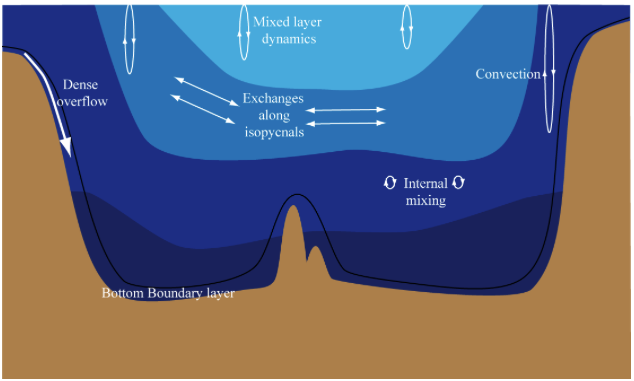
\includegraphics[width=0.8\linewidth]{images/ocean.png}
					\caption{Procesy małej skali uwzględnione jako $F_{diff}$. [7]}
				\end{center}
			\end{figure}

	
	
\end{frame}

\begin{frame}
	\frametitle{Modelowanie kriosfery}
	Własności kriosfery:
	\begin{itemize}
		\item Śnieg i lód mają wysokie albedo - są istotne w globalnym bilansie ciepła. 
		\item Zwiększają wymianę ciepła i gazów pomiędzy oceanami a atmosferą.
	\end{itemize}
\begin{block}{Śnieg i lód}
\[ \rho_c c_{pc} \frac{\partial T_c}{\partial t} = k_c \frac{\partial^2 T_c}{\partial z^2}	
\]	
\end{block}
\begin{block}{Dynamika lodu morskiego}
\[ m\frac{d\vec{u_i}}{dt	} = \vec{\tau_{ai}} + \vec{\tau_{wi}} -m\vec{f}e_z\times\vec{u_i} - mg\vec{\nabla}\mu + \vec{F_{int}} 
\]	
\end{block}

	
\end{frame}
\begin{frame}
	\frametitle{Modelowanie kriosfery}
				\begin{figure}[h]
				\begin{center}
					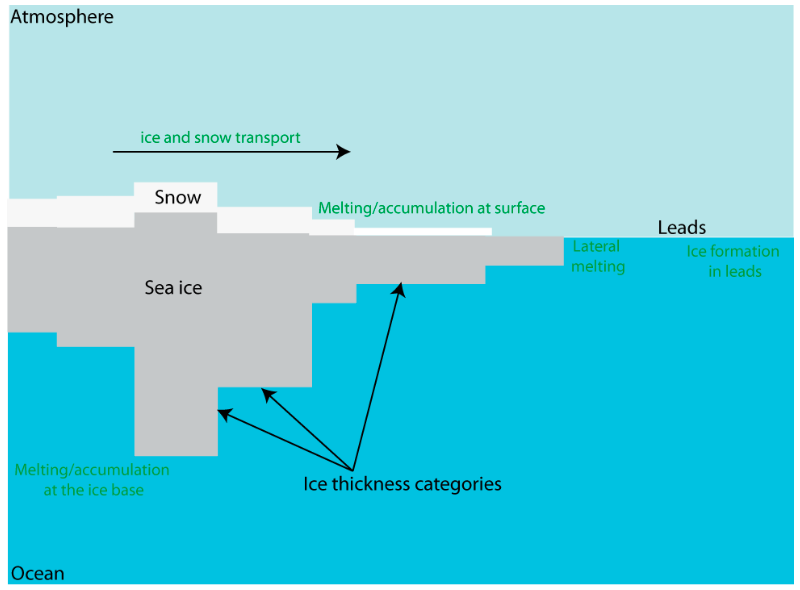
\includegraphics[width=0.8\linewidth]{images/ice.png}
					\caption{Główne procesy lodu morskiego. [7]}
				\end{center}
			\end{figure}
	
\end{frame}
\begin{frame}
	\frametitle{Powierzchnia lądowa}
			\begin{figure}[h]
				\begin{center}
					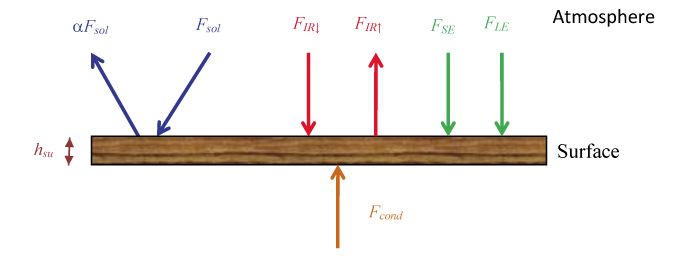
\includegraphics[width=0.8\linewidth]{images/lad.png}
					\caption{Wymiana ciepła powierzchni lądowej. [7]}
				\end{center}
			\end{figure}
	\begin{block}{Bilans ciepła}
		\[ \rho c_p h_{su} \frac{\partial T_s}{\partial t} = (1-\alpha)F_{sol} + F_{IR\downarrow} + F_{IR\uparrow} + F_{SE} + L_f E + F_{cond}
		\]
	\end{block}
	
	
\end{frame}
%-------------------------Atmosfera------------------------------%




\begin{frame}
	\frametitle{Połączenie powyższych składników}
	\begin{figure}[h]
		\begin{center}
			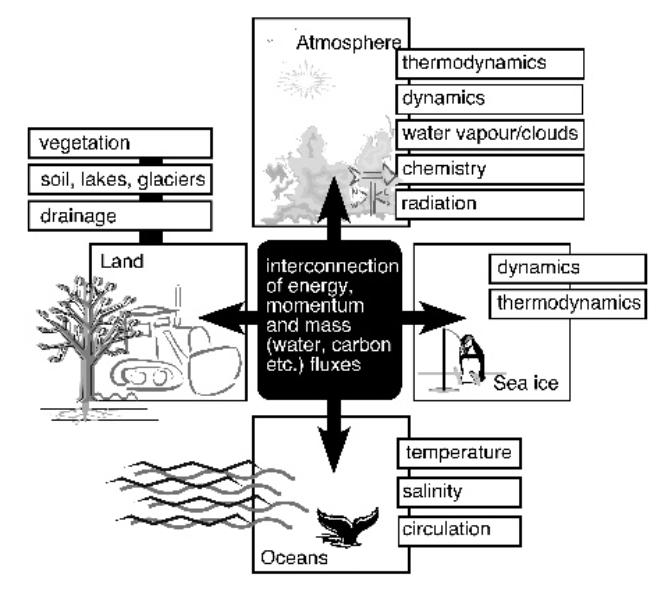
\includegraphics[width=0.6\linewidth]{images/Figure6.png}
			\caption{Wymiana wielkości fizycznych pomiędzy składowymi modelu. [1]}
		\end{center}
	\end{figure}
\end{frame}


%-------------------------MARCIN------------------------------%


\begin{frame}
	\frametitle{Jednowymiarowy EBM(energy balance model)}	
	\begin{figure}[h]
		\begin{center}
			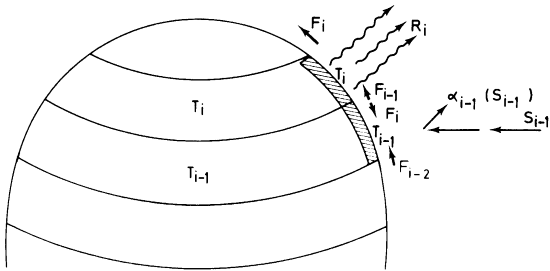
\includegraphics[width=0.7\linewidth]{images/1D_EBM.png}
			\caption{Schemat jednowymiarowego modelu bilansu energii.\cite{b3}}
		\end{center}
	\end{figure}
\end{frame}



\begin{frame}
	\frametitle{Jednowymiarowy RCM(radiative-convective model)}	
	\begin{figure}[h]
		\begin{center}
			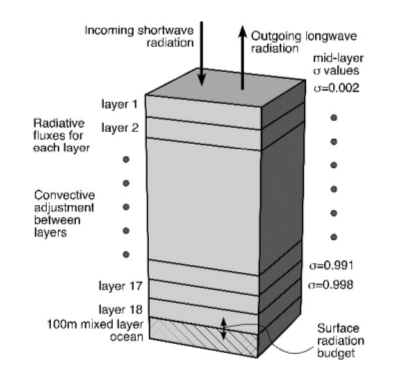
\includegraphics[width=0.6\linewidth]{images/1D_RC.png}
			\caption{Schemat jednowymiarowego modelu radiacyjno-konwekcyjnego.\cite{b1}}
		\end{center}
	\end{figure}
\end{frame}






\begin{frame}
	\frametitle{Przykład dwuwymiarowego modelu SD}
	
	\begin{figure}[h]
		\begin{center}
			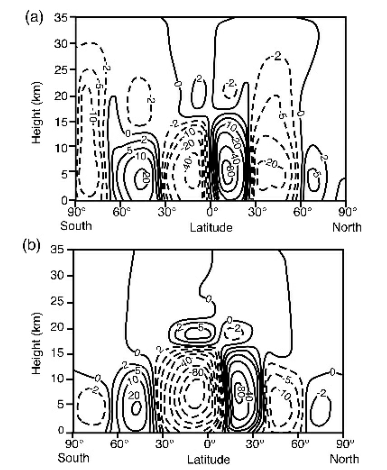
\includegraphics[width=0.4\linewidth]{images/2D_model.png}
			\caption{Rysunek przedstawia średni roczny przepływ masy. a) obserwowany, b) przewidziany modelem\cite{b1}}
		\end{center}
	\end{figure}
	
\end{frame}
%zależńość od szerokości geograficznej oraz wysokości. implementuje podstawowe prawa (prawo zachowania momentu pędu, równowaga hydrostsatyczna, równowaga termodynamiczna, prawo ciągłości). średnie strefowe


\begin{frame}
	\frametitle{Implementacja modelu GCM}
	W celu implementacji naszych równań musimy im nadać wartości dyskretne.
	Modelujemy atmosferę, dzieląc ją na pudła.
	
	\begin{figure}[h]
		\begin{center}
			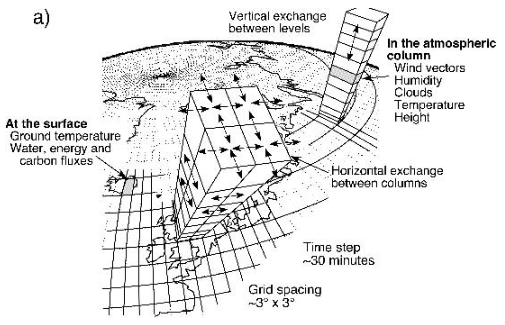
\includegraphics[width=0.7\linewidth]{images/box.png}
			\caption{Model podziału atmosfery na pudła. Dopuszczamy wymiany wertykalne i horyzontalne.\cite{b1}}
		\end{center}
	\end{figure}
	
	%zajrzec na strone 170 \cite{b1} spectral model - nie wiem czy mowic o tym
	%strona 187 opis 6 zmiennych i 6 rownan je opisujacych
\end{frame}


\begin{frame}
	\frametitle{Przykłady}
	\begin{figure}[h]
		\begin{center}
			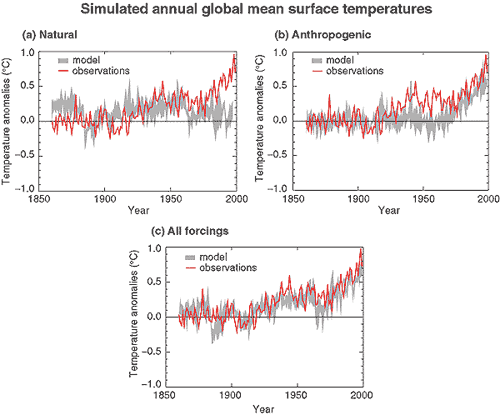
\includegraphics[width=0.7\linewidth]{images/przyklady/przyklad1.png}
			\caption{Porównanie średniej temperatury obserwowanej oraz wynikającej 
				z modelu.\cite{b5}}
		\end{center}
	\end{figure}
	
\end{frame}


\begin{frame}
	\frametitle{Przykłady}
	\begin{figure}[h]
		\begin{center}
			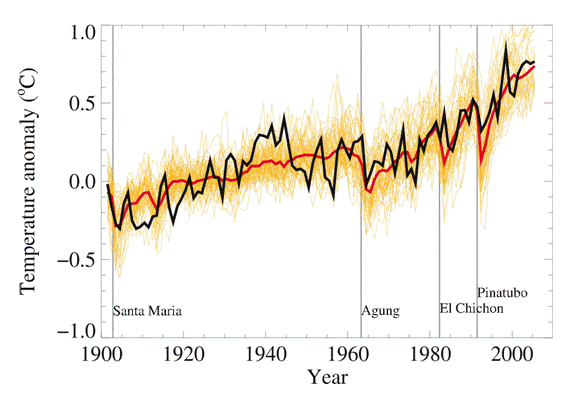
\includegraphics[width=0.7\linewidth]{images/przyklady/przyklad2.png}
			\caption{Wykres przedstawia anomalie temperatury w minionym stuleciu (z zaznaczonymi wybuchami wulkanów.)\cite{b4}}
		\end{center}
	\end{figure}
	
\end{frame}

\begin{frame}
	\frametitle{Przykłady}
	\begin{figure}[h]
		\begin{center}
			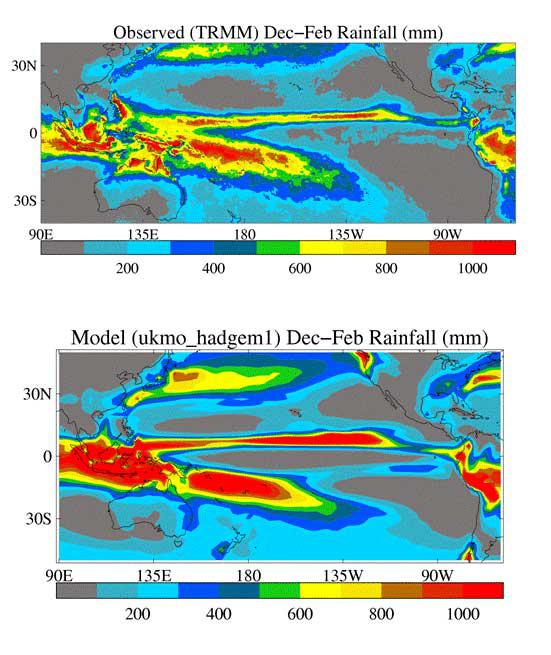
\includegraphics[width=0.45\linewidth]{images/przyklady/przyklad3.png}
			\caption{Porównanie opadów deszczu - modelowanych i obserwowanych. \cite{b4}}
		\end{center}
	\end{figure}
	
\end{frame}

\begin{frame}
	\frametitle{Przykłady}
	\begin{figure}[h]
		\begin{center}
			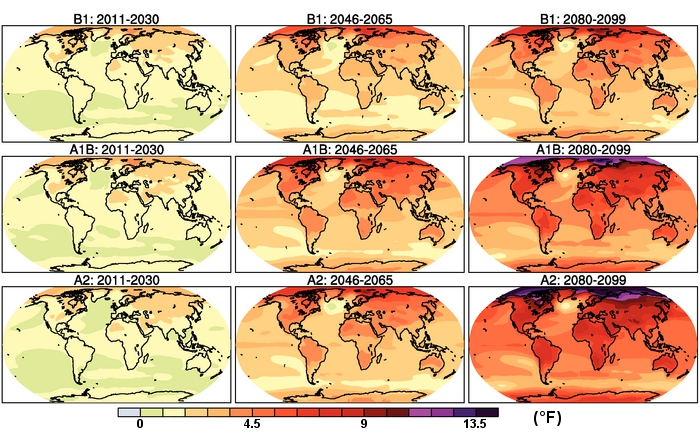
\includegraphics[width=0.7\linewidth]{images/przyklady/przyklad4.png}
			\caption{Przewidywany wzrost temperatury dla różnych prognoz wzrostu stężenia $CO^2$.\cite{b6}}
		\end{center}
	\end{figure}
	
\end{frame}




\begin{frame}
	\frametitle{Teoria Chaosu na przykładzie układu Lorentza}
	\begin{columns}
		\begin{column}{0.5\textwidth}	
			$\begin{cases} \dot{x} = \sigma(y-x)\\ \dot{y} =x(\rho-z)-y \\ \dot{z} = xy-\beta z \end{cases}$
		\end{column}
		\begin{column}{0.5\textwidth}
			\begin{figure}[h]
				\begin{center}
					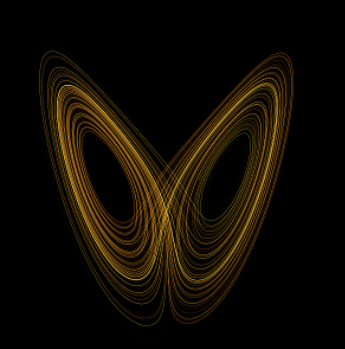
\includegraphics[width=0.7\linewidth]{images/motyl.png}
					\caption{Trajektoria układu Lorenza}
				\end{center}
			\end{figure}
		\end{column}
		
	\end{columns}
	
\end{frame}



\begin{frame}
	\frametitle{Bibliografia}
	\footnotesize{
		\begin{thebibliography}{99} % Beamer does not support BibTeX so references must be inserted manually as below
			\bibitem[1]{b1}[1] K.McGuffie, A. Henderson-Sellers
			\newblock A Climate Modelling Primer
			\newblock John Wiley \& Sons, Chichester, wydanie trzecie, 2005
			
			\bibitem[2]{b2}[2] E. Boeker, R. Grondelle
			\newblock Fizyka środowiska
			\newblock PWN, Warszawa, 2002
			
			\bibitem[3]{b3}[3] https://www.e-education.psu.edu
			
			\bibitem[4]{b4}[4] https://www.niwa.co.nz
			
			\bibitem[5]{b5}[5] http://www.skepticalscience.com
			
			\bibitem[6]{b6}[6] http://www.epa.gov
			
		\end{thebibliography}
	}
\end{frame}


\begin{frame}
	\Huge{\centerline{The End}}
\end{frame}
%KONIEC


\begin{comment}

\begin{frame}
	\frametitle{Plan prezentacji}
	\begin{enumerate}
		\item Co to jest klimat.
		\item Ważne pojęcia.
		\item Model zerowymiarowy - rozgrzewka (???).
		\item Modelowane zjawiska fizyczne (atmosfera, ocean ...).
		\item Sprzężenia zwrotne i parametryzacja.
		\item Rodzaje modeli + streszczenie.
		\item Implementacja GCM.
	\end{enumerate}
\end{frame}


\begin{frame}
	\frametitle{Modele 1D/2D/3D}
	\begin{enumerate}
		\item Model 1D:
		\begin{itemize}
			\item Model RC (radiative-convectiv model). %s.131
			
			\item One-dimensional EBM (energy balance model). %s.95
			%zależny od szerokości geograficznej, zmiana albedo, wymiana ciepła z sąsiadami, średnia temperatura strefowa
		\end{itemize}
		
		\item Model 2D:
		\begin{itemize}
			\item Two-dimensional SD (statistical dynamical) climate model.
			%height in the atmosphere and latitude
			%zonally averaged values
		\end{itemize}
		
		\item Model 3D:
		\begin{itemize}
			\item GCM (general circulation model)
		\end{itemize}
	\end{enumerate}
	
\end{frame}



\begin{frame}
	\frametitle{Przykłady zjawisk wpływających na globalne ocieplenie}

	\textbf{Zjawiska mogące wzmagać globalne ocieplenie:}
	\begin{enumerate}
		\item Topienie się lodów i śniegów.
		
		\item Zwiększenie ilości pary wodnej w powietrzu. 
		($t_a^{'}\nearrow; a_a^{'}\searrow$).
		
		\item Wzrost zachmurzenia.
		
		\item Wzrost $CO^2$ (mniejsza absorpcja przez oceany,
		szybszy rozkład materii).
		
		\item Szybszy wzrost roślin i zmiana albedo.

	\end{enumerate}

\end{frame}


\begin{frame}
	\frametitle{Przykłady zjawisk wpływających na globalne ocieplenie}
	
	\textbf{Zjawiska mogące osłabiać globalne ocieplenie:}
	
	\begin{enumerate}
		
		\item Wzrost zawartości pary wodnej (średni spadek temperatury
		z wysokością maleje).
		
		\item Wzmożony rozwój alg we wszystkich wodach (użycie $CO^2$ 
		do fotosyntezy).
		
	\end{enumerate}
	
\end{frame}



\begin{frame}
	\frametitle{Opóźnienie czasowe ze względu na obecność oceanów}
	
	\begin{itemize}
		\item Wysoka pojemność cieplna wody.
		
		\item Duża powierzchnia wód na Ziemi.
		
		\item Powolne zmiany temperatury.
	
	\end{itemize}
	
	\begin{block}{Zmiana temperatury w wyniku wymuszenia radiacyjnego}
		\[\Delta T_s(t) = G_f\Delta I
		\]
	\end{block}
	
	\begin{block}{Ta sama zmiana po uwzględnieniu opóźnienia czasowego}
		\[\Delta T_s(t) = G_f\Delta I(1-\exp^{-t/\tau _e})
		\]
	\end{block}
	
	$\tau _e \approx 50-100$ lat
	
\end{frame}







\begin{frame}
	\frametitle{TODO}
	\begin{itemize}
		\item Zmienne w modelach
		\item Opisać modele 0/1/2/3 wymiarowe
		\item Problemy i sprzężenia zwrotne
		\item Modelowanie atmosfery, oceanu, lądu, innych
	\end{itemize}
\end{frame}



\begin{frame}
	\frametitle{Hipotetyczne przykłady}
	\begin{itemize}
		\item \textit{Współczesna Ziemia.} ($a=0,30, T_s=288K$)
		\item \textit{Biała Ziemia.} ($a = 0,50;T_s=268K$)
		\item \textit{Zima nuklearna.} ($a=0,35; T_s=284K$)
	\end{itemize}
	
\end{frame}



\end{comment}





\end{document} 